% =====================================================================
%  CHƯƠNG 4. KẾT QUẢ THỰC NGHIỆM CỦA MÔ HÌNH
%  Nguồn số: runs/paper_queue/UNIFIED.json (1 chương trình đo, 3 seed),
%            runs/paper_queue/BASELINES_TABLE.md (tham số, GFLOPs),
%            runs/paper_queue/FLIGHT.json (92 khung bay thật, bootstrap).
% =====================================================================
\chapter{Kết quả thực nghiệm của mô hình}
\label{chap:ketqua}

Chương này trình bày kết quả đánh giá mô hình theo đúng giao thức ở Chương~\ref{chap:dulieu}. Mọi số liệu trên VisDrone-person được đo bằng một chương trình duy nhất; các cột có rung là trung bình $\pm$ độ lệch chuẩn qua ba hạt giống. Chương gồm bốn phần: tác dụng của huấn luyện nhận biết rung cùng các đối chứng; tính tổng quát và giới hạn của phương pháp; so sánh với năm mô hình nhẹ công khai; và kiểm chứng trên dữ liệu bay thật.

\section{Kết quả chính và các thí nghiệm đối chứng}
\label{sec:ketquachinh}

\begin{table}[H]
\centering
\caption{Kết quả trên VisDrone-person, ảnh $640\times640$. Trong mỗi khối, các dòng chỉ khác nhau đúng một yếu tố và dùng chung lịch trình, learning rate và phép tăng cường. Cột có rung: trung bình $\pm$ độ lệch chuẩn qua 3 hạt giống}
\label{tab:ketquachinh}
\footnotesize
\setlength{\tabcolsep}{3.2pt}
\renewcommand{\arraystretch}{1.18}
\resizebox{\textwidth}{!}{%
\begin{tabular}{@{}lccc|cccc@{}}
\toprule
 & \multicolumn{3}{c|}{\textbf{Ảnh sạch}} & \multicolumn{4}{c}{\textbf{Khi rung (AP@[.50:.95])}}\\
\textbf{Mô hình} & \textbf{AP} & \textbf{AP$_{50}$} & \textbf{AP$_{75}$} & \textbf{Mức 1} & \textbf{Mức 2} & \textbf{Mức 3} & \textbf{retain (\%)}\\
\midrule
\multicolumn{8}{@{}l}{\textit{SteadyDet-N (1,17 triệu tham số; 4,6 GFLOPs)}}\\
\quad Gốc & 0,1892 & 0,5127 & 0,0811 & \ms{0,0792}{0,0026} & \ms{0,0123}{0,0013} & \ms{0,0040}{0,0005} & \ms{16,8}{0,7}\\
\quad + 120 epoch không rung & 0,1823 & 0,4984 & 0,0762 & \ms{0,0761}{0,0028} & \ms{0,0125}{0,0005} & \ms{0,0040}{0,0005} & \ms{16,9}{0,7}\\
\quad + ràng buộc nhất quán & 0,1746 & 0,4837 & 0,0728 & \ms{0,1098}{0,0010} & \ms{0,0392}{0,0021} & \ms{0,0081}{0,0011} & \ms{30,0}{0,6}\\
\quad \textbf{+ huấn luyện nhận biết rung} & 0,1708 & 0,4731 & 0,0715 & \textbf{\ms{0,1223}{0,0014}} & \textbf{\ms{0,0518}{0,0019}} & \textbf{\ms{0,0111}{0,0002}} & \textbf{\ms{36,2}{0,7}}\\
\midrule
\multicolumn{8}{@{}l}{\textit{SteadyDet-W (1,00 triệu tham số; 12,9 GFLOPs)}}\\
\quad Gốc & 0,2349 & 0,5800 & 0,1305 & \ms{0,1260}{0,0023} & \ms{0,0258}{0,0022} & \ms{0,0046}{0,0026} & \ms{22,2}{0,9}\\
\quad + ràng buộc nhất quán & 0,2207 & 0,5561 & 0,1202 & \ms{0,1309}{0,0026} & \ms{0,0580}{0,0007} & \ms{0,0132}{0,0016} & \ms{30,5}{0,6}\\
\quad \textbf{+ huấn luyện nhận biết rung} & 0,2219 & 0,5511 & 0,1279 & \textbf{\ms{0,1583}{0,0013}} & \textbf{\ms{0,0839}{0,0001}} & \textbf{\ms{0,0200}{0,0012}} & \textbf{\ms{39,4}{0,3}}\\
\midrule
\multicolumn{8}{@{}l}{\textit{YOLO11-n huấn luyện từ đầu trên cùng dữ liệu (2,59 triệu tham số; 6,4 GFLOPs)}}\\
\quad Gốc & 0,2588 & 0,5842 & 0,1839 & \ms{0,1398}{0,0057} & \ms{0,0248}{0,0022} & \ms{0,0052}{0,0021} & \ms{21,9}{1,1}\\
\quad + 120 epoch không rung & 0,2641 & 0,5897 & 0,1857 & \ms{0,1410}{0,0036} & \ms{0,0226}{0,0026} & \ms{0,0062}{0,0030} & \ms{21,4}{0,9}\\
\quad + huấn luyện nhận biết rung & 0,2579 & 0,5835 & 0,1806 & \ms{0,1384}{0,0037} & \ms{0,0227}{0,0017} & \ms{0,0055}{0,0026} & \ms{21,5}{0,8}\\
\bottomrule
\end{tabular}}
\end{table}

\subsection{Mọi bộ phát hiện nhỏ gọn đều sụp đổ khi rung}

Dòng đầu của Bảng~\ref{tab:ketquachinh} cho thấy mức độ nghiêm trọng của vấn đề. SteadyDet-N gốc đạt AP 0,1892 trên ảnh sạch nhưng chỉ còn 0,0123 ở mức rung 2, tức giữ lại 6,5\% độ chính xác ở đúng điều kiện bay tiến thông thường; tính trung bình ba mức, nó chỉ giữ được $16{,}8 \pm 0{,}7\%$. Mục~\ref{sec:sosanh} sẽ cho thấy đây không phải điểm yếu riêng của mô hình này: mọi mô hình đối chứng, từ 2,5 tới 32,8 triệu tham số, đều mất 74--83\% độ chính xác.

\subsection{Huấn luyện nhận biết rung tăng gấp đôi tỷ lệ giữ độ chính xác}

Tinh chỉnh với toán tử rung nâng retain của SteadyDet-N từ $16{,}8 \pm 0{,}7\%$ lên $36{,}2 \pm 0{,}7\%$, gấp 2,15 lần. Ở mức rung 2, AP tăng từ 0,0123 lên 0,0518, tức \textbf{tăng 4,2 lần}, và mô hình giữ được 30,3\% độ chính xác sạch thay vì 6,5\%. Cái giá phải trả là AP trên ảnh sạch giảm 9,7\% (từ 0,1892 xuống 0,1708). Với một hệ thống bay, đây là trao đổi có lợi: một bộ phát hiện kém hơn một phần mười khi đứng yên nhưng chính xác hơn bốn lần khi cánh quạt đang quay là bộ phát hiện hữu ích hơn. Chênh lệch retain giữa hai mô hình (19,3 điểm) lớn hơn khoảng 20 lần độ lệch chuẩn gộp của hai phép đo, nên không thể do ngẫu nhiên của giao thức đo.

\subsection{Đối chứng 1: tác dụng không đến từ việc huấn luyện thêm}

Vì phương pháp được áp dụng dưới dạng tinh chỉnh, mô hình nhận biết rung đã được huấn luyện thêm 120 epoch mà mô hình gốc không có. Thí nghiệm đối chứng tinh chỉnh đúng 120 epoch với cùng mọi thiết lập nhưng tắt toán tử rung cho retain $16{,}9 \pm 0{,}7\%$, nằm trong một độ lệch chuẩn so với mô hình gốc ($16{,}8 \pm 0{,}7\%$). Huấn luyện thêm không đóng góp gì cho độ bền. Tuy vậy, AP sạch có giảm nhẹ trong 120 epoch đó (0,1892 xuống 0,1823), nên khoảng một phần ba mức giảm AP sạch của mô hình nhận biết rung đến từ bản thân quá trình tinh chỉnh chứ không phải từ toán tử rung.

\subsection{Đối chứng 2: ràng buộc nhất quán kém hơn phương pháp đơn giản}

Kết quả này trái với kỳ vọng ban đầu của nhóm. Biến thể ràng buộc nhất quán theo phương trình~(\ref{eq:vibcons}) chỉ đạt retain $30{,}0 \pm 0{,}6\%$, thấp hơn phương pháp đơn giản 6,2 điểm phần trăm, khoảng chín lần độ lệch chuẩn của mỗi phép đo. Nó cũng kém hơn ở \textit{từng} mức rung tính theo AP tuyệt đối chứ không chỉ sau khi chuẩn hoá, trong khi tốn 1,8 lần thời gian huấn luyện. Cách giải thích của nhóm là: ở biến thể này, hàm mất mát phát hiện chỉ được tính trên nhánh sạch, nên mạng không bao giờ bị yêu cầu \textit{phát hiện} trên ảnh nhoè; nó chỉ bị yêu cầu làm cho dự đoán trên ảnh nhoè giống dự đoán trên ảnh sạch. Yêu cầu này yếu hơn và có thể được thoả mãn bằng cách làm cả hai dự đoán bớt chắc chắn. Phương pháp đơn giản đặt ảnh nhoè trực tiếp đối diện với nhãn. Đây là cách giải thích hợp lý chứ chưa được chứng minh bằng thí nghiệm riêng.

\begin{figure}[H]
\centering
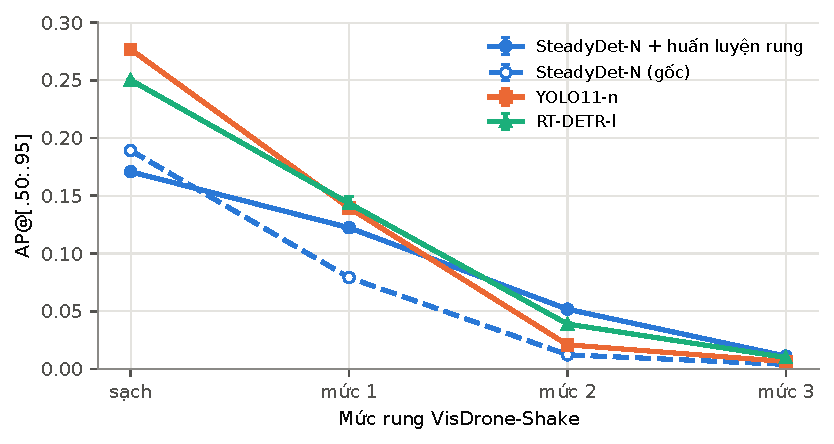
\includegraphics[width=0.94\textwidth]{duong_cong_rung.pdf}
\caption{AP@[.50:.95] theo mức rung. Mô hình gốc (nét đứt) có AP sạch cao hơn nhưng giảm nhanh nhất; sau huấn luyện nhận biết rung (nét liền xanh), SteadyDet-N vượt YOLO11-n và RT-DETR-l từ mức rung 2. Thanh sai số: độ lệch chuẩn qua 3 hạt giống}
\label{fig:duongcong}
\end{figure}

\section{Tính tổng quát và giới hạn của phương pháp}
\label{sec:tongquat}

\subsection{Lặp lại trên một kiến trúc khác}

Một phương pháp chỉ có tác dụng trên đúng một kiến trúc thì khó phân biệt với một sự tương tác may mắn. Khối giữa của Bảng~\ref{tab:ketquachinh} lặp lại thí nghiệm trên SteadyDet-W, mô hình có nhánh $P_2$ đầy đủ, head năm lớp tích chập và chi phí gấp 2,8 lần, mà không chỉnh lại siêu tham số nào. Retain tăng từ $22{,}2 \pm 0{,}9\%$ lên $39{,}4 \pm 0{,}3\%$, tức +17,2 điểm so với +19,3 điểm ở SteadyDet-N; biến thể ràng buộc nhất quán lại một lần nữa kém hơn ($30{,}5 \pm 0{,}6\%$). Chiều hướng, độ lớn và thứ tự giữa hai biến thể đều được tái lập trên một mạng có độ rộng, độ sâu và thiết kế head khác.

\subsection{Không có tác dụng trên YOLO11-n}

Khối dưới cùng áp dụng đúng quy trình cho YOLO11-n và kết quả là không có thay đổi: retain từ $21{,}9 \pm 1{,}1\%$ thành $21{,}5 \pm 0{,}8\%$, đối chứng không rung $21{,}4 \pm 0{,}9\%$. Trên checkpoint YOLO11-n được huấn luyện sẵn trên COCO, phương pháp cho $20{,}1\%$ thành $20{,}1\%$, còn biến thể nhất quán cho $19{,}2\%$. Nhật ký huấn luyện xác nhận toán tử rung đã thực sự được áp dụng. Nhóm đã kiểm tra ba giả thuyết và cả ba đều bị bác bỏ:
\begin{itemize}
\item \textit{Do huấn luyện sẵn trên COCO}: nếu mô hình đã có sẵn đặc trưng chịu được nhoè thì không còn gì để học. Huấn luyện YOLO11-n từ khởi tạo ngẫu nhiên vẫn cho kết quả không đổi, và checkpoint huấn luyện sẵn lại là bản \textit{kém} bền hơn (20,1\% so với 21,9\%).
\item \textit{Do kích thước vật}: có thể chỉ mức bước 4 mới hưởng lợi. Nhưng khi tách riêng vật nhỏ, mức tăng của SteadyDet-N là +18,7 điểm so với +19,3 điểm tổng thể, và gần như mọi người trong tập đều là vật nhỏ với cả hai họ mô hình (AP$_s$ của YOLO11-n là 0,2741 trên AP 0,2768).
\item \textit{Do khoảng trống còn lại}: SteadyDet-W bắt đầu từ $22{,}2 \pm 0{,}9\%$ và YOLO11-n từ đầu bắt đầu từ $21{,}9 \pm 1{,}1\%$, gần như cùng điểm xuất phát, nhưng một mô hình tăng 17,2 điểm, mô hình kia không tăng.
\end{itemize}
Nguyên nhân còn lại nằm ở kiến trúc hoặc hàm mất mát mà hai mô hình của đề tài có chung còn YOLO11-n thì không: mức bước 4, hàm mất mát NWD kết hợp CIoU, QFL, và hồi quy hộp trực tiếp thay vì theo phân phối. Một mô hình không phản hồi không đủ để tách các yếu tố này, nên đề tài phát biểu kết luận đúng phạm vi bằng chứng: phương pháp cho mức tăng lớn và tái lập được trên họ kiến trúc của đề tài, và không có tác dụng trên mô hình ngoài họ đã thử.

Kết quả âm này cũng có một vai trò quan trọng: nó làm cho phép so sánh ở mục sau trở nên công bằng. Vì phương pháp không nâng được YOLO11-n, việc so sánh ``SteadyDet-N có xử lý'' với ``YOLO11-n không xử lý'' không phải là so với một đối thủ bị làm yếu đi.

\section{So sánh với các mô hình phát hiện nhẹ}
\label{sec:sosanh}

\begin{table}[H]
\centering
\caption{So sánh với năm mô hình công khai trên VisDrone-person, mọi dòng đo bằng cùng một chương trình. mCP: AP@[.50:.95] trung bình ba mức rung, tức độ chính xác \textit{khi bay}. Các mô hình YOLO và RT-DETR khởi tạo từ trọng số huấn luyện sẵn trên COCO, còn SteadyDet huấn luyện từ đầu, điều này có lợi cho mô hình đối chứng}
\label{tab:sosanh}
\small
\setlength{\tabcolsep}{4pt}
\renewcommand{\arraystretch}{1.15}
\begin{tabular}{@{}lcccccc@{}}
\toprule
\textbf{Mô hình} & \textbf{Tham số (M)} & \textbf{GFLOPs} & \textbf{AP$_{50}$} & \textbf{AP} & \textbf{mCP} & \textbf{retain (\%)}\\
\midrule
RT-DETR-l~\cite{zhao2024rtdetr} & 32,81 & 108,0 & 0,5909 & 0,2502$^{\dagger}$ & 0,0641 & \ms{25,6}{1,1}\\
YOLOv10-n~\cite{wang2024yolov10} & 2,71 & 8,4 & 0,6043 & 0,2730 & 0,0538 & \ms{19,7}{1,4}\\
YOLOv8-n~\cite{ultralytics} & 3,01 & 8,2 & 0,6033 & 0,2684 & 0,0522 & \ms{19,5}{0,8}\\
YOLO26-n~\cite{ultralytics} & 2,50 & 5,8 & 0,5898 & 0,2675 & 0,0507 & \ms{19,0}{1,0}\\
YOLO11-n~\cite{ultralytics} & 2,59 & 6,4 & \textbf{0,6119} & \textbf{0,2768} & 0,0557 & \ms{20,1}{1,2}\\
\quad + huấn luyện nhận biết rung & 2,59 & 6,4 & 0,6057 & 0,2700 & 0,0542 & \ms{20,1}{1,3}\\
\midrule
SteadyDet-W (gốc) & 1,00 & 12,9 & 0,5800 & 0,2349 & 0,0521 & \ms{22,2}{0,9}\\
\quad \textbf{+ huấn luyện nhận biết rung} & 1,00 & 12,9 & 0,5511 & 0,2219 & \textbf{0,0874} & \textbf{\ms{39,4}{0,3}}\\
SteadyDet-N (gốc) & \textbf{1,17} & \textbf{4,6} & 0,5127 & 0,1892 & 0,0318 & \ms{16,8}{0,7}\\
\quad + ràng buộc nhất quán & 1,17 & 4,6 & 0,4837 & 0,1746 & 0,0524 & \ms{30,0}{0,6}\\
\quad \textbf{+ huấn luyện nhận biết rung} & \textbf{1,17} & \textbf{4,6} & 0,4731 & 0,1708 & \textbf{0,0617} & \textbf{\ms{36,2}{0,7}}\\
\bottomrule
\multicolumn{7}{@{}p{0.98\textwidth}@{}}{\footnotesize $^{\dagger}$ Bộ tiền xử lý gốc của RT-DETR kéo giãn ảnh thay vì đệm xám; trong đường xử lý chung, AP sạch của nó bị kéo xuống (chương trình gốc cho 0,3340). mCP và retain là tỷ số trong cùng một đường xử lý nên không bị ảnh hưởng.}\\
\end{tabular}
\end{table}

\subsection{Trên ảnh sạch, SteadyDet-N không dẫn đầu}

Cả bốn mô hình YOLO bản nano đều có AP sạch cao hơn SteadyDet-N, và đề tài không né tránh điều đó. Việc các mô hình đối chứng được khởi tạo từ trọng số huấn luyện sẵn trên COCO là một yếu tố, nhưng khoảng cách lớn hơn mức mà yếu tố này có thể giải thích. Hiệu quả tính toán cũng không bù được: 4,6 GFLOPs so với 5,8 GFLOPs của mô hình đối chứng rẻ nhất (YOLO26-n) chỉ tiết kiệm 21\%. Nếu chỉ xét benchmark trên ảnh sạch, SteadyDet-N thua.

\subsection{Khi rung, thứ hạng đảo ngược}

Cột mCP xếp hạng bảng gần như ngược với cột AP sạch. SteadyDet-N có huấn luyện nhận biết rung đạt mCP 0,0617, cao hơn mô hình đối chứng nhỏ tốt nhất là YOLO11-n (0,0557), trong khi chỉ dùng 45\% số tham số và 72\% chi phí tính toán của nó. \textbf{SteadyDet-N vượt cả bốn mô hình YOLO bản nano về độ chính xác khi bay.}

RT-DETR-l có mCP trung bình cao hơn SteadyDet-N (0,0641 so với 0,0617), nhưng không phải ở điều kiện quan trọng nhất. Ở mức rung 2, tương ứng bay tiến thông thường, RT-DETR-l đạt $0{,}0389 \pm 0{,}0014$ còn SteadyDet-N đạt $0{,}0518 \pm 0{,}0019$, chênh lệch khoảng 5,5 lần độ lệch chuẩn gộp, trong khi RT-DETR-l có số tham số gấp 28 lần và chi phí gấp 23 lần. Ở mức 3, hai mô hình nằm trong phạm vi nhiễu ($0{,}0100 \pm 0{,}0017$ so với $0{,}0111 \pm 0{,}0002$), nên đề tài không kết luận thứ tự ở mức này. So với YOLO11-n ở mức 2, SteadyDet-N hơn 2,5 lần (0,0518 so với 0,0210).

SteadyDet-W có huấn luyện nhận biết rung dẫn đầu toàn bảng với mCP 0,0874. Tuy vậy, đề tài chọn SteadyDet-N làm mô hình chính vì trên nền tảng đích, ràng buộc chặt nhất là chi phí tính toán chứ không phải số tham số: mô hình, bộ theo vết và bộ điều khiển phải cùng vừa một khung thời gian. Tính trên mỗi GFLOP, thứ tự rất rõ ràng: SteadyDet-N đạt 0,0134 mCP/GFLOP, so với 0,0087 của YOLO11-n và 0,0068 của SteadyDet-W.

\begin{figure}[H]
\centering
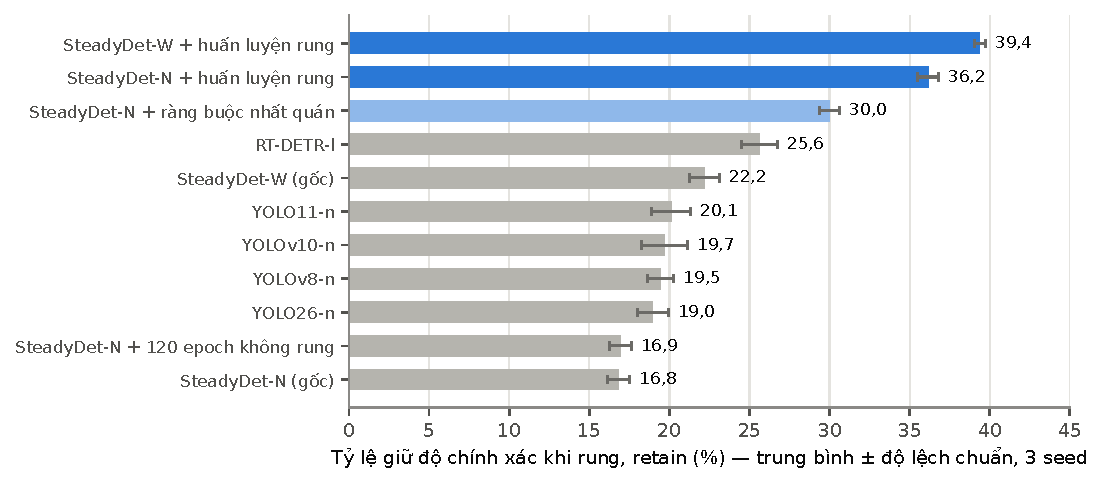
\includegraphics[width=0.94\textwidth]{retain.pdf}
\caption{Tỷ lệ giữ độ chính xác khi rung của mọi mô hình. Bốn thế hệ YOLO bản nano nằm sát nhau ở 19--20\% dù khác nhau về kiến trúc; hai mô hình của đề tài sau huấn luyện nhận biết rung đứng đầu}
\label{fig:retain}
\end{figure}

\subsection{Độ bền không phải là sản phẩm phụ của độ chính xác}

Hình~\ref{fig:danhdoi} biểu diễn AP sạch theo mCP. Các mô hình công khai tập trung ở góc phải dưới: độ chính xác sạch cao hơn nhưng không bền hơn; bốn thế hệ YOLO trải dài bốn năm và ba trường phái thiết kế nhưng retain chỉ cách nhau khoảng một điểm phần trăm. RT-DETR-l đạt 25,6\% nhờ số tham số gấp 28 lần. Hendrycks và Dietterich đã ghi nhận hiện tượng tương tự với mô hình phân loại ImageNet~\cite{hendrycks2019imagenetc}: độ bền tương đối gần như không cải thiện qua nhiều năm tiến bộ kiến trúc. Kết quả của đề tài cho thấy điều này cũng đúng với bộ phát hiện nhẹ trên ảnh UAV. Hệ quả thực tiễn là \textbf{độ bền phải được đo và tối ưu riêng}; các mũi tên trong hình cho thấy thay đổi phân phối huấn luyện mang lại mức tăng độ bền lớn với mức giảm độ chính xác sạch nhỏ.

\begin{figure}[H]
\centering
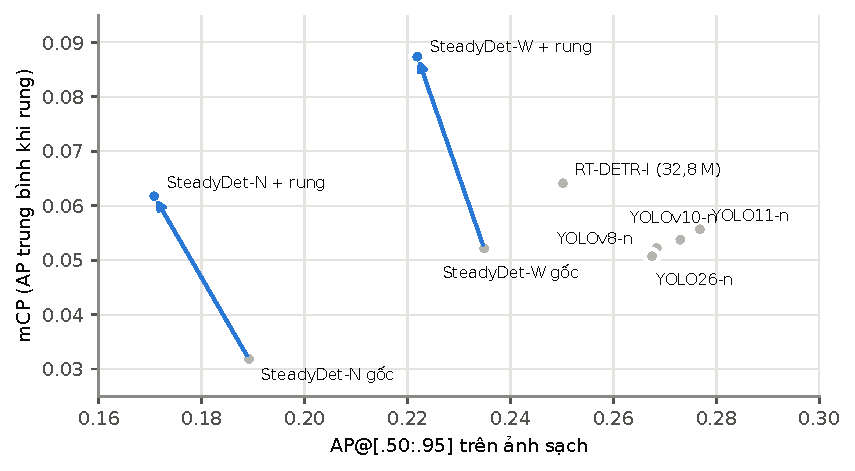
\includegraphics[width=0.94\textwidth]{danh_doi.pdf}
\caption{AP trên ảnh sạch và mCP khi rung, mỗi điểm là một mô hình. Mũi tên xanh: tác dụng của huấn luyện nhận biết rung trên hai mô hình của đề tài}
\label{fig:danhdoi}
\end{figure}

\section{Kiểm chứng trên dữ liệu bay thật}
\label{sec:baythat}

Mọi kết quả ở trên dựa trên suy giảm mô phỏng. Mục này dùng 92 khung hình bay thật ở độ cao khoảng 6\,m, nơi nhoè do chính máy bay tạo ra. Sáu mô hình SteadyDet-N có cùng kiến trúc được so sánh theo hai trục độc lập: dữ liệu huấn luyện (có hay không có COCO-person) và cách xử lý rung.

\begin{table}[H]
\centering
\caption{Kết quả trên 92 khung hình bay thật ($\approx$6\,m), cùng chương trình đo. Trong mỗi nhóm, ba mô hình giống hệt kiến trúc và chỉ khác cách xử lý rung}
\label{tab:baythat}
\small
\renewcommand{\arraystretch}{1.15}
\begin{tabular}{@{}llcccc@{}}
\toprule
\textbf{Dữ liệu huấn luyện} & \textbf{Xử lý rung} & \textbf{AP$_{50}$} & \textbf{AP} & \textbf{AP$_{75}$} & \textbf{AR$_{100}$}\\
\midrule
VisDrone + COCO-person & không & 0,7613 & 0,3369 & 0,1448 & 0,5076\\
VisDrone + COCO-person & huấn luyện nhận biết rung & 0,7747 & 0,3792 & 0,2583 & \textbf{0,5315}\\
VisDrone + COCO-person & ràng buộc nhất quán & \textbf{0,8798} & \textbf{0,3885} & \textbf{0,2620} & 0,5087\\
\midrule
Chỉ VisDrone & không & 0,1435 & 0,0547 & 0,0166 & 0,4315\\
Chỉ VisDrone & huấn luyện nhận biết rung & 0,0579 & 0,0207 & 0,0076 & 0,4076\\
Chỉ VisDrone & ràng buộc nhất quán & 0,0909 & 0,0283 & 0,0093 & 0,3772\\
\bottomrule
\end{tabular}
\end{table}

\begin{figure}[H]
\centering
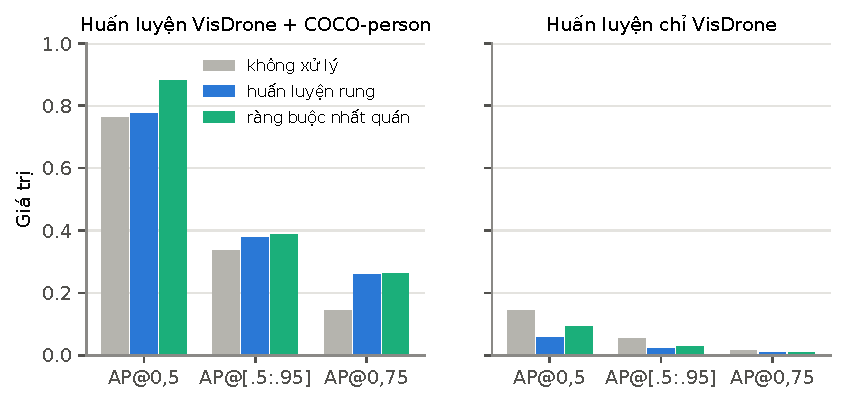
\includegraphics[width=0.94\textwidth]{bay_that.pdf}
\caption{Kết quả trên dữ liệu bay thật theo nhóm dữ liệu huấn luyện. Nhóm có COCO-person (trái) chính xác gấp nhiều lần nhóm chỉ VisDrone (phải); trong nhóm có COCO, cả hai cách xử lý rung làm AP@0,75 tăng gần gấp đôi}
\label{fig:baythat}
\end{figure}

\subsection{Cả hai cách xử lý rung đều có tác dụng trên rung thật}

Trong nhóm mô hình phù hợp với miền này (có COCO-person), cả hai cách xử lý đều cải thiện theo cùng một kiểu. AP@0,75 tăng từ 0,1448 lên 0,2583 với huấn luyện nhận biết rung và 0,2620 với ràng buộc nhất quán, tức tăng tương đối 78\% và 81\% ở độ khít hộp, trong khi recall gần như không đổi (0,5076 thành 0,5315 và 0,5087). Mô hình không tìm thấy thêm người; nó đặt hộp khít hơn quanh những người đã tìm thấy, đúng dấu hiệu mong đợi nếu mô hình học được cách nhìn xuyên qua nhoè.

Để kiểm tra ý nghĩa thống kê trên 92 khung, đề tài lấy mẫu lại khung hình 1.000 lần theo cặp. Khoảng tin cậy 95\% của hiệu so với mô hình không xử lý:
\begin{itemize}
\item huấn luyện nhận biết rung: AP +0,042 [+0,011; +0,074], AP@0,75 +0,108 [+0,010; +0,211];
\item ràng buộc nhất quán: AP +0,051 [+0,012; +0,087], AP@0,75 +0,110 [+0,012; +0,214], AP@0,5 +0,119 [+0,071; +0,173].
\end{itemize}
Mọi khoảng tin cậy trên đều không chứa 0, nên cả hai cách xử lý thực sự tốt hơn mô hình không xử lý trên dữ liệu này. Hai cách xử lý chỉ tách nhau ở AP@0,5 (+0,106 [+0,058; +0,161] nghiêng về ràng buộc nhất quán), còn hiệu AP và AP@0,75 giữa chúng đều chứa 0. Thứ tự ở AP@0,5 ngược với thứ tự trên VisDrone-Shake. Với một người, một cảnh và một độ cao, dữ liệu này không đủ để quyết định thứ tự nào tổng quát hơn; câu trả lời cần một tập bay lớn hơn.

\subsection{Chọn dữ liệu theo miền triển khai, không theo benchmark}

Thêm COCO-person làm AP@0,5 trên dữ liệu bay thật tăng 5,3 lần (0,1435 lên 0,7613), trong khi trên VisDrone-val cùng thay đổi này lại \textit{làm giảm} AP@0,5 (0,5127 xuống 0,5016). Phân tích chi tiết giải thích cơ chế: mô hình chỉ học VisDrone vẫn có recall khá (0,4315), tức vẫn thấy người, nhưng định vị sụp đổ (AP@0,75 chỉ 0,0166) vì chưa từng được học trên người chiếm phần lớn khung hình. Nếu chọn dữ liệu huấn luyện dựa trên benchmark, nhóm sẽ chọn đúng mô hình sai. Với bài toán bám theo người ở cự ly gần, dữ liệu huấn luyện phải khớp với dải độ cao triển khai.

Trong nhóm chỉ VisDrone, thứ tự đảo ngược (AP@0,5 giảm từ 0,1435 xuống 0,0909 và 0,0579). Cả ba mô hình này đều thất bại ở miền bay thấp, nên so sánh giữa chúng là so sánh giữa các cách thất bại: làm cho biểu diễn bền trước nhoè chỉ có ích khi biểu diễn đó vốn đã phù hợp. Huấn luyện nhận biết rung là phương pháp tăng độ bền, không phải phương pháp thích nghi miền.

\section{Thảo luận}

Bốn kết luận chính rút ra từ chương này:
\begin{enumerate}
\item Rung là điều kiện luôn có khi bay, và dưới một giao thức đo thống nhất, mọi bộ phát hiện nhỏ gọn đều mất phần lớn độ chính xác. Vấn đề thuộc về điều kiện vận hành chứ không thuộc về một kiến trúc cụ thể.
\item Huấn luyện nhận biết rung tăng retain của SteadyDet-N từ 16,8\% lên 36,2\% và AP ở mức rung 2 lên 4,2 lần, không tốn chi phí suy luận; đối chứng xác nhận tác dụng không đến từ việc huấn luyện thêm.
\item Kiến trúc và phương pháp huấn luyện đều cần thiết: SteadyDet-N không xử lý đứng cuối bảng về mCP, còn phương pháp áp dụng lên YOLO11-n không có tác dụng. Chỉ khi kết hợp cả hai, mô hình nhỏ nhất và rẻ nhất mới vượt cả bốn mô hình YOLO bản nano khi rung.
\item Trên dữ liệu bay thật, xử lý rung làm hộp khít hơn rõ rệt, và dữ liệu huấn luyện phù hợp miền triển khai quan trọng hơn thứ hạng trên benchmark.
\end{enumerate}

Các giới hạn cần nêu rõ: toán tử rung là mô hình mô phỏng, tham số được chọn để bao quát điều kiện bay chứ chưa hiệu chuẩn theo phổ gia tốc đo trên chính khung máy bay; mỗi cấu hình chỉ được huấn luyện một lần nên thanh sai số phản ánh biến động của phép đo chứ chưa phản ánh biến động của huấn luyện; tập bay thật mới có một người, một cảnh, một độ cao. Các giới hạn này được đưa vào phần kiến nghị.
